\documentclass{article}
\usepackage[utf8]{inputenc}
\usepackage{pythonhighlight}
\usepackage{amsmath}
\usepackage{graphicx}
\usepackage{listings}
\usepackage{subcaption}
\usepackage{lscape}
\usepackage{hyperref}

\begin{document}

\begin{titlepage}
   \vspace*{\stretch{1.0}}
   \begin{center}
      \Large\textbf{PHY408: Time Series Analysis}\\
      \Large\textbf{Final Term Paper}\\ 
      \vspace{1cm}
      \large{April 12, 2018} \\ 
      \vspace{2cm}
      \large{Saila Shama} \\
	\end{center}
   \vspace*{\stretch{2.0}}
\end{titlepage}

\tableofcontents

\newpage
\section{Introduction}
Two datasets were explored for this report. The first one was the daily rainfall data in Melbourne from 1981 to 1990 as reported by the \href{http://www.bom.gov.au/?ref=logo}{Australian Bureau of Meteorology.} The specific location and station from which this dataset was obtained is unknown since the dataset was downloaded from a third-party site, \href{http://www.statsci.org/data/oz/melbrain.html}{statsci.org}. The second dataset was also downloaded from the \href{http://www.statsci.org/data/oz/melbtemp.html}{same site} and pertains to the daily maximum and minimum temperatures in Melbourne from 1981 to 1990.


The analysis performed on these datasets were mostly for exploratory purposes. In order to look for trends and periodicities in Melbourne's rainfall and temperature data, spectrum analysis and autocorrelation was performed. Then, in hopes of finding a relationship between temperature and rainfall data, a cross-correlation analysis was performed. 

\newpage
\section{Data Processing}

The following steps were taken to process the data. 
\begin{enumerate}
	\item \textbf{NaN values}: The NaN values in each data set were replaced by using linear extrapolation. This was done so as to avoid the fourier transform of these time-series being all NaN entries.
	\begin{python}
		def remove_nan(x):
		xi = np.arange(len(x))
		
		mask = np.isfinite(x)
		xfiltered = np.interp(xi, xi[mask], x[mask])
		
		return xfiltered
	\end{python}

	\item \textbf{Data length:} Since the temperature dataset excluded the two leap year dates from 1984 and 1988, its length was shorter than that of the rainfall dataset. As such, the two leap year entries were also removed from the rainfall data. However, after doing that the rainfall time-series was still one-entry longer than the temperature-time series. This did not make sense as the total number of days (excluding leap days) between 1981 and 1990 is 3650 whereas the length of the rainfall time-series was 3650. In order to resolve this issue, the last entry of the rain-falll time series was also deleted. 
	
	\begin{python}
	  # delete leap year days from 1984 and 1988
		# remove indices 365*3+31+29 = 1155, 365*7+1+31+29 = 2616
		# assume last data point is extra so remove that as well
		rain_data = np.delete(rain_data, [1155,2616, len(rain_data)-1])
	\end{python}

	\item \textbf{Trend}: Each of the time-series was detrended using \texttt{scipy.signal.detrend} function before performing fourier analysis.
	
	\item \textbf{Centering}: The mean of each of the time-series was subtracted from their respective time-series.
	
\end{enumerate}


\newpage
\section{Analysis}

\subsection{Raw Data}
The raw data is visualized in Figure \ref{ref:raw_data}

\begin{figure}[h!]
	\caption{Plot of raw data}
	\label{ref:raw_data}
	\begin{subfigure}{\textwidth}
		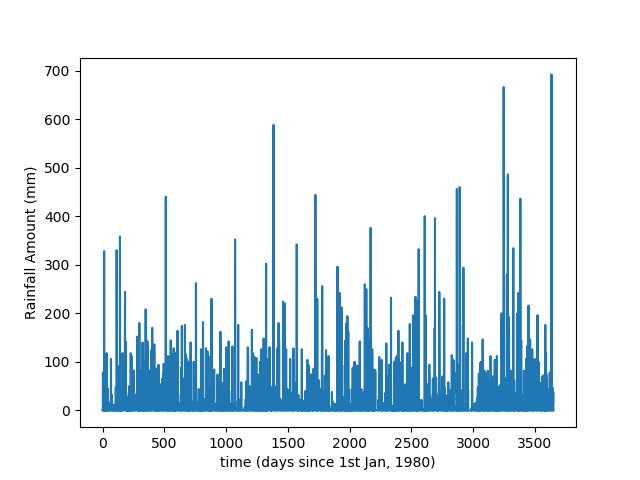
\includegraphics[width=\linewidth, height=6cm]{figures/raw_data_rain.png} 
		\caption{Rainfall data}
		\label{fig:raw_data_rain}
	\end{subfigure}
	\begin{subfigure}{\textwidth}
		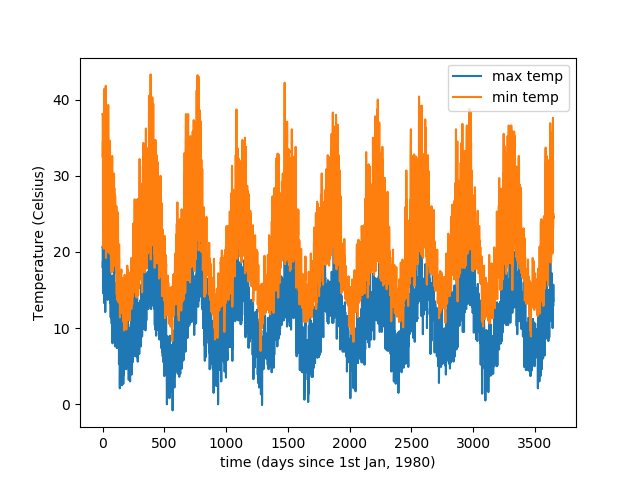
\includegraphics[width=\linewidth, height=6cm]{figures/raw_data_temp.png}
		\caption{Temperature data}	
		\label{fig:raw_data_temp}
	\end{subfigure}
\end{figure}

\newpage
\subsection{Power Spectrum Analysis}
The power spectra of each of time-series is shown in Figure \ref{fig:spectrum_analysis}
\begin{figure}[h!]
	\caption{Power spectra of each dataset}
	\begin{subfigure}{\textwidth}
		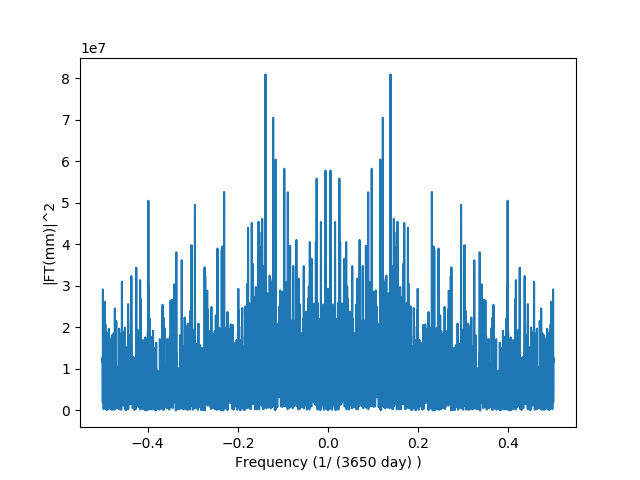
\includegraphics[width=\linewidth, height=4.5cm]{figures/power_spectrum_rainfall.png} 
		\caption{Power Spectrum of rainfall data}
		\label{fig:power_spectrum_rainfall}
	\end{subfigure}
	\begin{subfigure}{\textwidth}
		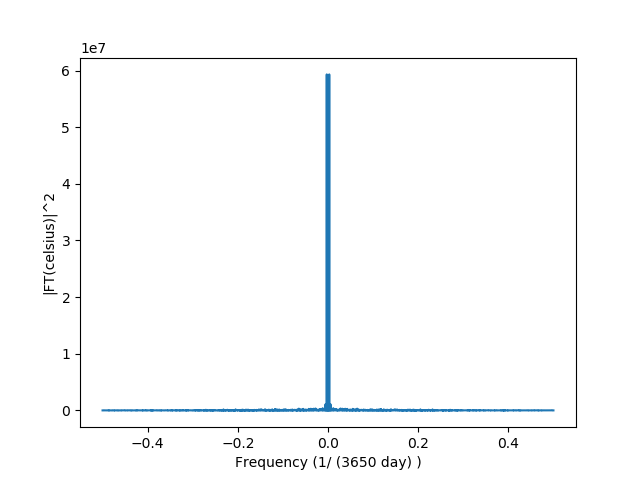
\includegraphics[width=\linewidth, height=4.5cm]{figures/power_spectrum_max_temp.png}
		\caption{Power spectrum of temperature data (maximum)}	
		\label{fig:power_spectrum_max_temp}
	\end{subfigure}
	\begin{subfigure}{\textwidth}
		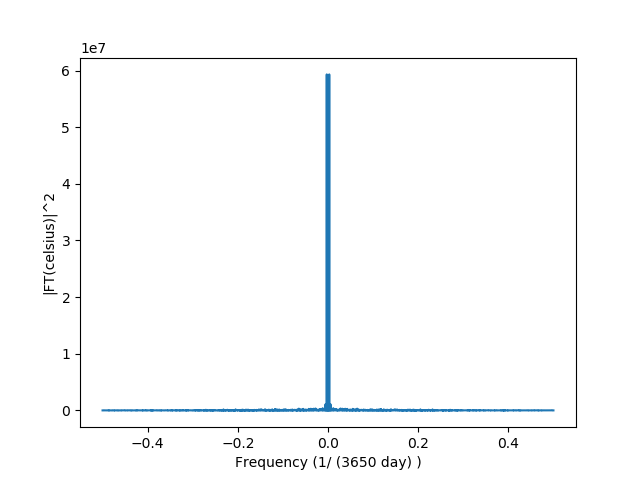
\includegraphics[width=\linewidth, height=4.5cm]{figures/power_spectrum_max_temp.png}
		\caption{Power spectrum of temperature data (minimum)}	
		\label{fig:power_spectrum_min_temp}
	\end{subfigure}
	\label{fig:spectrum_analysis}
\end{figure}

\newpage
\subsection{Autocorrelation Analysis}
The autocorrelation of each of the time-series was found using Python's \texttt{scipy.signal.corrleate} function and is shown in Figure \ref{fig:autocorrelation_analysis}

\begin{figure}[h!]
	\caption{Autocorrelation of each dataset}
	\begin{subfigure}{\textwidth}
		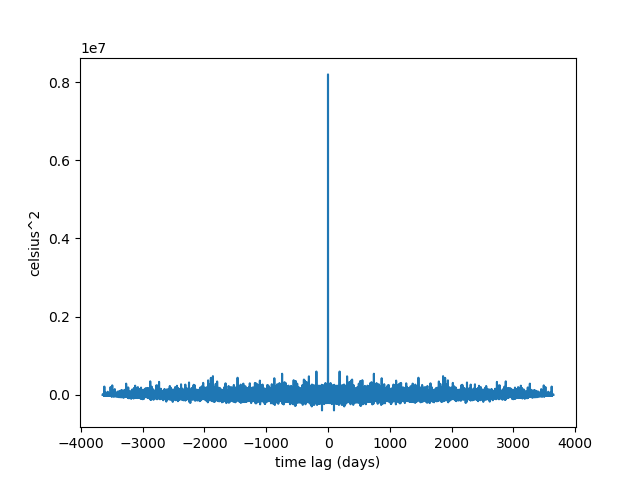
\includegraphics[width=\linewidth, height=4.5cm]{figures/auto_correlation_rainfall.png} 
		\caption{Autocorrelation of rainfall data}
		\label{fig:acm_rainfall}
	\end{subfigure}
	\begin{subfigure}{\textwidth}
		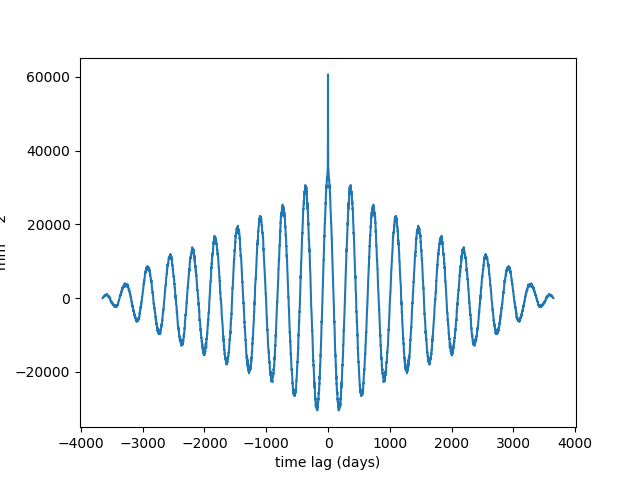
\includegraphics[width=\linewidth, height=4.5cm]{figures/auto_correlation_max_temp.png}
		\caption{Autocorrelation of temperature data (maximum)}	
		\label{fig:ac_max_temp}
	\end{subfigure}
	\begin{subfigure}{\textwidth}
		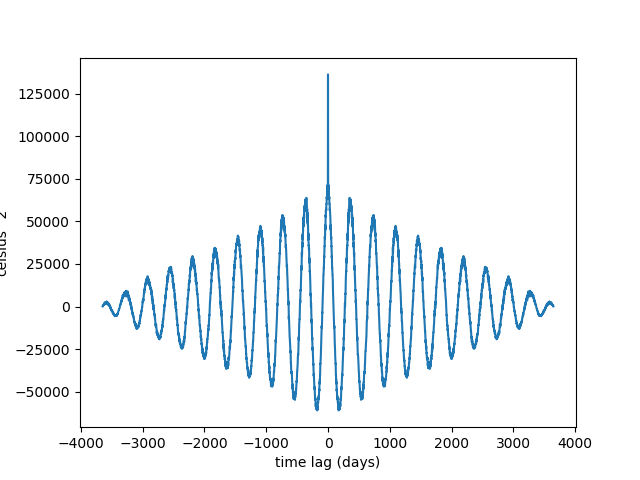
\includegraphics[width=\linewidth, height=4.5cm]{figures/auto_correlation_min_temp.png}
		\caption{Autocorrelation of temperature data (minimum)}	
		\label{fig:ac_min_temp}
	\end{subfigure}
	\label{fig:autocorrelation_analysis}
\end{figure}

\newpage
\subsection{Cross-correlation Analysis}
The cross-correlation between each of the time series data was found in two ways. One by using Python's \texttt{numpy.fft} package and the other using Python's \texttt{scipy.signal.correlate} function. The former is shown below in Figure \ref{fig:cross-correlation analysis_np.fft} while the latter can be viewed in the appendix in \ref{fig:cross-correlation analysis scipy.signal.correlate}. 

\begin{figure}[h!]
	\caption{Cross-correlation between each time-series using np.fft package}
	\begin{subfigure}{\textwidth}
		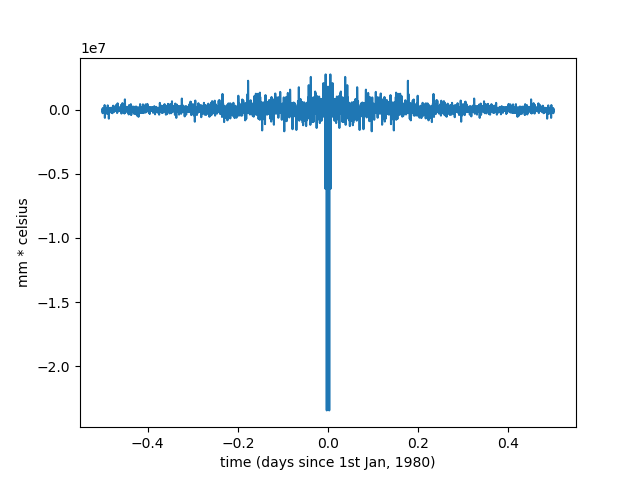
\includegraphics[width=\linewidth, height=4cm]{figures/old/cross_correlation_max_temp_rainfall.png} 
		\caption{Cross-correlation between maximum temperature and rainfall }
		\label{fig:cc_max_temp_rainfall_np}
	\end{subfigure}
	\begin{subfigure}{\textwidth}
		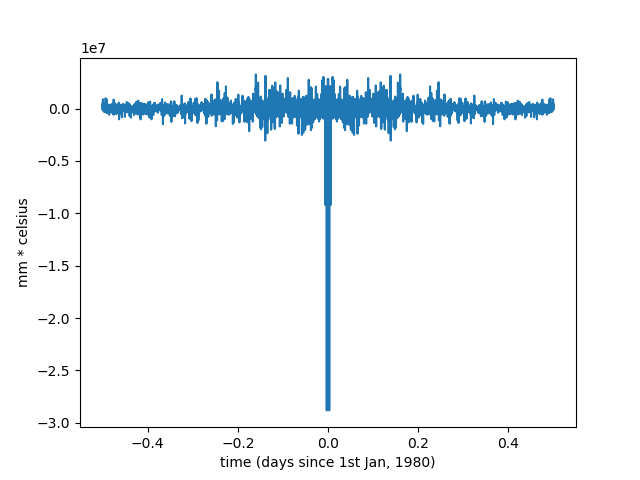
\includegraphics[width=\linewidth, height=4cm]{figures/old/cross_correlation_min_temp_rainfall.png}
		\caption{Cross correlation between minimum temperature and rainfall}	
		\label{fig:cc_min_temp_rainfall_np}
	\end{subfigure}
	\begin{subfigure}{\textwidth}
		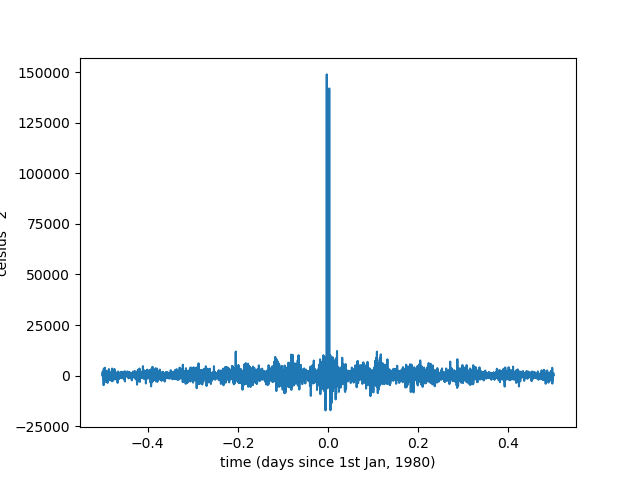
\includegraphics[width=\linewidth, height=4cm]{figures/old/cross_correlation_max_temp_min_temp.png}
		\caption{Cross correlation between maximum temperature and minimum temperature}	
		\label{fig:cc_max_temp_min_temp_np}
	\end{subfigure}
	\label{fig:cross-correlation analysis_np.fft}
\end{figure}

\newpage
\section{Discussion}
With reference to \ref{fig:raw_data_temp}, immediately we can see periodicities in the temperature data. We also see an obvious correlation between the maximum temperature and minimum temperatures. This is further supported by the power spectra of these temperature series in \ref{fig:power_spectrum_max_temp} and \ref{fig:power_spectrum_min_temp}. There is clearly a peak at the center frequency, implying that the temperature time-series is periodic with a certain frequency. That the frequency happens to be zero informs us that the temperature remains constant through out the years, but since we know that is not true, the frequency axis of the power spectra is probably erroneous. 


In contrast to the temperature time-series, from \ref{fig:raw_data_rain}, periodicities in the rainfall data seem obscure and non-existent. However, upon viewing its power spectrum in \ref{fig:power_spectrum_rainfall}, we notice two peaks that are slightly higher than the rest. This was found to be at -0.138 and +0.138, however since the frequency axis is erroneous these values provide no more information other than the fact that there exist two frequencies at which the power spectrum achieves identical maximum values. 

In order to supplement findings about periodicity from the power spectra, autocorrelation graphs for each of the time-series were also plotted, as shown in \ref{fig:autocorrelation_analysis}. In Figures \ref{fig:ac_max_temp} and \ref{fig:ac_min_temp}, we see sharp peaks on top of the sinusoidal peak at the center of the graph. Perhaps this means that the time series repeates itself over a period other than the trivial period (its own length). The peak in the autocorrelation graph of the rainfall data as seen in \ref{fig:acm_rainfall} seems to imply nothing more than the fact that the data is most alike itself when completely overlapped. 

In Figure \ref{fig:cc_max_temp_rainfall_np} and \ref{fig:cc_min_temp_rainfall_np}, we see that the cross-correlation between the two temperatures and rainfall data peak negatively. This implies that when temperature decreases, rainfall increases and vice versa. And finally, the cross correlation between the two temperature data in Figure \ref{fig:cc_max_temp_min_temp_np} has a distinct positive peak as expected. 





\newpage
\section*{Appendix}
\subsection*{Cross-correlation using scipy package}
\begin{figure}[h!]
	\caption{Cross-correlation between each time-series using scipy.signal.correlate}
	\begin{subfigure}{\textwidth}
		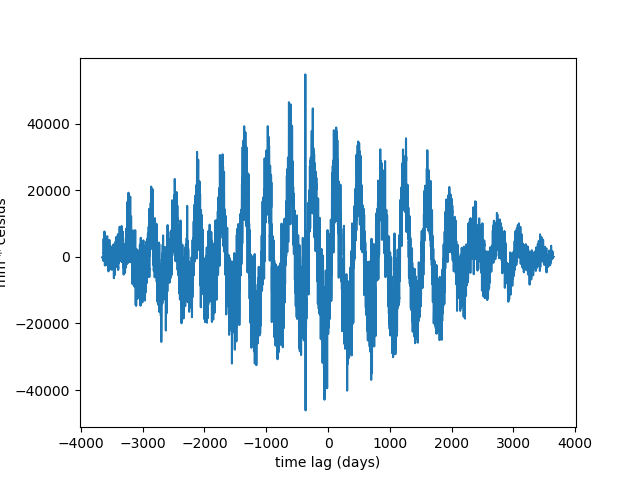
\includegraphics[width=\linewidth, height=4.5cm]{figures/cross_correlation_max_temp_rainfall.png} 
		\caption{Cross-correlation beween maximum temperature and rainfall }
		\label{fig:cc_max_temp_rainfall_scipy.correlate}
	\end{subfigure}
	\begin{subfigure}{\textwidth}
		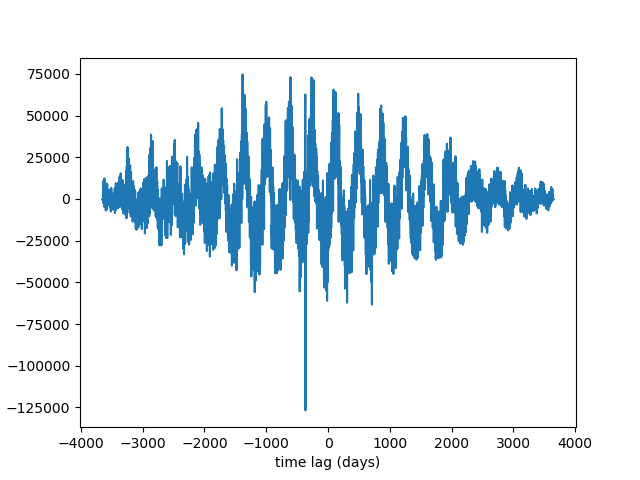
\includegraphics[width=\linewidth, height=4.5cm]{figures/cross_correlation_min_temp_rainfall.png}
		\caption{Cross correlation between minimum temperature and rainfall}	
		\label{fig:cc_min_temp_rainfall_scipy.correlate}
	\end{subfigure}
	\begin{subfigure}{\textwidth}
		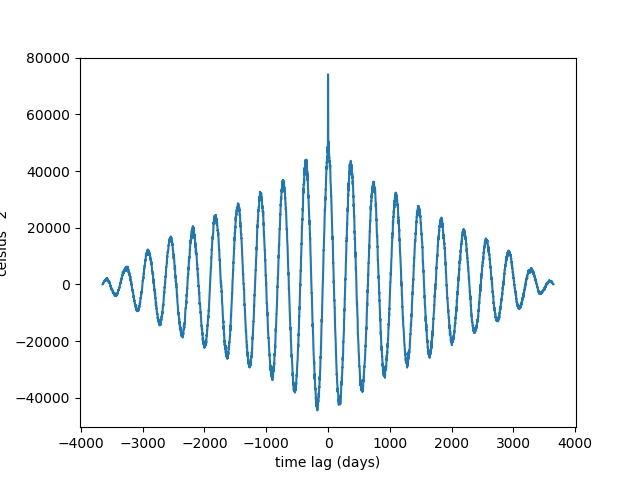
\includegraphics[width=\linewidth, height=4.5cm]{figures/cross_correlation_max_temp_min_temp.png}
		\caption{Cross correlation between maximum temperature and minimum temperature}	
		\label{fig:cc_max_temp_min_temp_scipy.correlate}
	\end{subfigure}
	\label{fig:cross-correlation analysis scipy.signal.correlate}
\end{figure}
\newpage

\newpage
\subsection*{Python script}
The script used to obtain the results of the dataset is included below.
\begin{python}
import numpy as np
import matplotlib.pyplot as plt
from scipy.signal import detrend, correlate

def get_fft(x, dt):
x_ft = np.fft.fftshift(np.fft.fft(x)*dt)
freq_axis = np.fft.fftshift(np.fft.fftfreq(len(x), dt))

return freq_axis, x_ft


def get_ifft(x, dt):
ifft = np.fft.fftshift(np.fft.ifft(np.fft.fftshift(x / dt)))
time_axis = np.fft.fftshift(np.fft.fftfreq(len(x), dt))
return time_axis, ifft

def remove_nan(x):
xi = np.arange(len(x))

mask = np.isfinite(x)
xfiltered = np.interp(xi, xi[mask], x[mask])

return xfiltered


if __name__ == "__main__":

###################### LOAD DATA #############################

rain_data = np.genfromtxt("melbrain.txt") #3653 observations
temp_data_max = np.genfromtxt("melbtemp.txt")[:,0] #10 x 365 = 3650 observations.
temp_data_min = np.genfromtxt("melbtemp.txt")[:,1]


###################### PROCESS DATA #############################

#fix dimension problem for cross-correlation
# delete leap year days between in 1984 and 1988 from rain data
# remove indices 365*3+31+29 = 1155, 365*7+1+31+29 = 2616
# assume last data point is extra so remove that as well
rain_data = np.delete(rain_data, [1155,2616, len(rain_data)-1])

#remove Nan by linear extrapolation so that FT doesn't all give NaN values
rain_data = remove_nan(rain_data)
temp_data_max = remove_nan(temp_data_max)
temp_data_min = remove_nan(temp_data_min)

np.savetxt("processed_rain_data.txt", rain_data)

#################### PLOT RAW DATA #######################

plt.plot(rain_data, label="rainfall")
plt.xlabel("time (days since 1st Jan, 1980)")
plt.ylabel("Rainfall Amount (mm)")
plt.savefig("figures/raw_data_rain.png")
plt.clf()

plt.plot(temp_data_max, label="max temp")
plt.plot(temp_data_min, label="min temp")
plt.legend()
plt.xlabel("time (days since 1st Jan, 1980)")
plt.ylabel("Temperature (Celsius)")
plt.savefig("figures/raw_data_temp.png")
plt.clf()

################## FOURIER ANAYSIS #####################

#detrend data
rain_data_detrended = detrend(rain_data)
temp_data_max_detrended = detrend(temp_data_max)
temp_data_min_detrended = detrend(temp_data_min)

rain_data_detrended_centered = rain_data_detrended - np.mean(rain_data_detrended)
temp_data_max_detrended_centered = temp_data_max_detrended - np.mean(temp_data_max_detrended)
temp_data_min_detrended_centered = temp_data_min_detrended - np.mean(temp_data_min_detrended)

dt = 1
freq_axis_rain, rain_data_ft = get_fft(rain_data_detrended_centered, dt)
freq_axis_temp_max, temp_data_max_ft = get_fft(temp_data_max_detrended_centered, dt)
freq_axis_temp_min, temp_data_min_ft = get_fft(temp_data_min_detrended_centered, dt)


plt.plot(freq_axis_rain, rain_data_ft, label = "rainfall ft")
plt.xlabel("Frequency (1/ (3650 day) )")
plt.ylabel("FT(mm)")
plt.savefig("figures/freq_spectrum_rainfall.png")
plt.clf()

plt.plot(freq_axis_temp_max, temp_data_max_ft, label ="temp_max")
plt.xlabel("Frequency (1/ (3650 day) )")
plt.ylabel("FT(degree celsius)")
plt.savefig("figures/freq_spectrum_max_temp.png")
plt.clf()

plt.plot(freq_axis_temp_min, temp_data_max_ft, label = "temp_min")
plt.xlabel("Frequency (1/ (3650 day) )")
plt.ylabel("FT(degree celsius)")
plt.savefig("figures/freq_spectrum_min_temp.png")
plt.clf()

################ POWER SPECTRUM ANAYSIS #####################

rainfall_power_spectrum = np.abs(rain_data_ft) ** 2
plt.plot(freq_axis_rain, rainfall_power_spectrum, label="rainfall power spectrum")
plt.xlabel("Frequency (1/ (3650 day) )")
plt.ylabel("|FT(mm)|^2")
plt.savefig("figures/power_spectrum_rainfall.png")
plt.clf()

temp_max_power_spectrum = np.abs(temp_data_max_ft) ** 2
plt.plot(freq_axis_rain, temp_max_power_spectrum, label="temp max power spectrum")
plt.xlabel("Frequency (1/ (3650 day) )")
plt.ylabel("|FT(celsius)|^2")
plt.savefig("figures/power_spectrum_max_temp.png")
plt.clf()

temp_min_power_spectrum = np.abs(temp_data_min_ft) ** 2
plt.plot(freq_axis_rain, temp_min_power_spectrum, label="temp min power spectrum")
plt.xlabel("Frequency (1/ (3650 day) )")
plt.ylabel("|FT(celsius)|^2")
plt.savefig("figures/power_spectrum_min_temp.png")
plt.clf()

##### get frequencies of peaks ######
print(freq_axis_rain[np.where(rainfall_power_spectrum == max(rainfall_power_spectrum))])

################ AUTO CORRELATION ANAYSIS #################
# auto_correlation_ft = temp_data_max_ft.conjugate() * temp_data_max_ft
# time_axis, auto_correlation = get_ifft(auto_correlation_ft, dt)
# plt.plot(time_axis, auto_correlation, label="auto_correlation_temp_max")

    auto_correlation = correlate(temp_data_max_detrended_centered, temp_data_max_detrended_centered)
time_axis = np.arange(-len(auto_correlation)/2, len(auto_correlation)/2, 1)

plt.plot(time_axis, auto_correlation, label="auto_correlation_temp_max")
plt.xlabel("time lag (days)")
plt.ylabel("mm ^ 2")
plt.savefig("figures/auto_correlation_max_temp.png")
plt.clf()

auto_correlation = correlate(temp_data_min_detrended_centered, temp_data_min_detrended_centered)
time_axis = np.arange(-len(auto_correlation) / 2, len(auto_correlation) / 2, 1)
plt.plot(time_axis, auto_correlation, label="auto_correlation_temp_min")
plt.xlabel("time lag (days)")
plt.ylabel("celsius^2")
plt.savefig("figures/auto_correlation_min_temp.png")
plt.clf()

auto_correlation = correlate(rain_data_detrended_centered, rain_data_detrended_centered)
time_axis = np.arange(-len(auto_correlation) / 2, len(auto_correlation) / 2, 1)
plt.plot(time_axis, auto_correlation, label="auto_correlation_rainfall")
plt.xlabel("time lag (days)")
plt.ylabel("celsius^2")
plt.savefig("figures/auto_correlation_rainfall.png")
plt.clf()


################ CROSS CORRELATION ANAYSIS ###################
#uncomment to replicate to obtain Figure 4
# cross_correlation_ft = temp_data_max_ft.conjugate() * rain_data_ft
# time_axis, cross_correlation = get_ifft(cross_correlation_ft,dt)
#plt.plot(time_axis, cross_correlation, label = "cross_correlation_max_temp_rainfall")

cross_correlation = correlate(temp_data_max_detrended_centered, rain_data_detrended_centered)
time_axis = np.arange(-len(cross_correlation) / 2, len(cross_correlation) / 2, 1)
plt.plot(time_axis, cross_correlation, label = "cross_correlation_max_temp_rainfall")
plt.xlabel("time lag (days)")
plt.ylabel("mm * celsius")
plt.savefig("figures/cross_correlation_max_temp_rainfall.png")
plt.clf()

cross_correlation_ft = correlate(temp_data_min_detrended_centered, rain_data_detrended_centered)
time_axis = np.arange(-len(cross_correlation) / 2, len(cross_correlation) / 2, 1)
plt.plot(time_axis,cross_correlation, label = "cross_correlation_min_temp_rainfall")
plt.xlabel("time lag (days)")
plt.ylabel("mm * celsius")
plt.savefig("figures/cross_correlation_min_temp_rainfall.png")
plt.clf()

cross_correlation_ft = correlate(temp_data_max_detrended_centered, temp_data_min_detrended)
time_axis = np.arange(-len(cross_correlation) / 2, len(cross_correlation) / 2, 1)
plt.plot(time_axis,cross_correlation, label = "cross_correlation_max_temp_min_temp")
plt.xlabel("time lag (days)")
plt.ylabel("celsius^2")
plt.savefig("figures/cross_correlation_max_temp_min_temp.png")
plt.clf()
	
\end{python}


\end{document}
